
\section{Use-Cases}

\subsection{Use-case Diagram}
Her ses aktør usecase diagrammet for det realistiske system:
\begin{figure}[H]
\centering
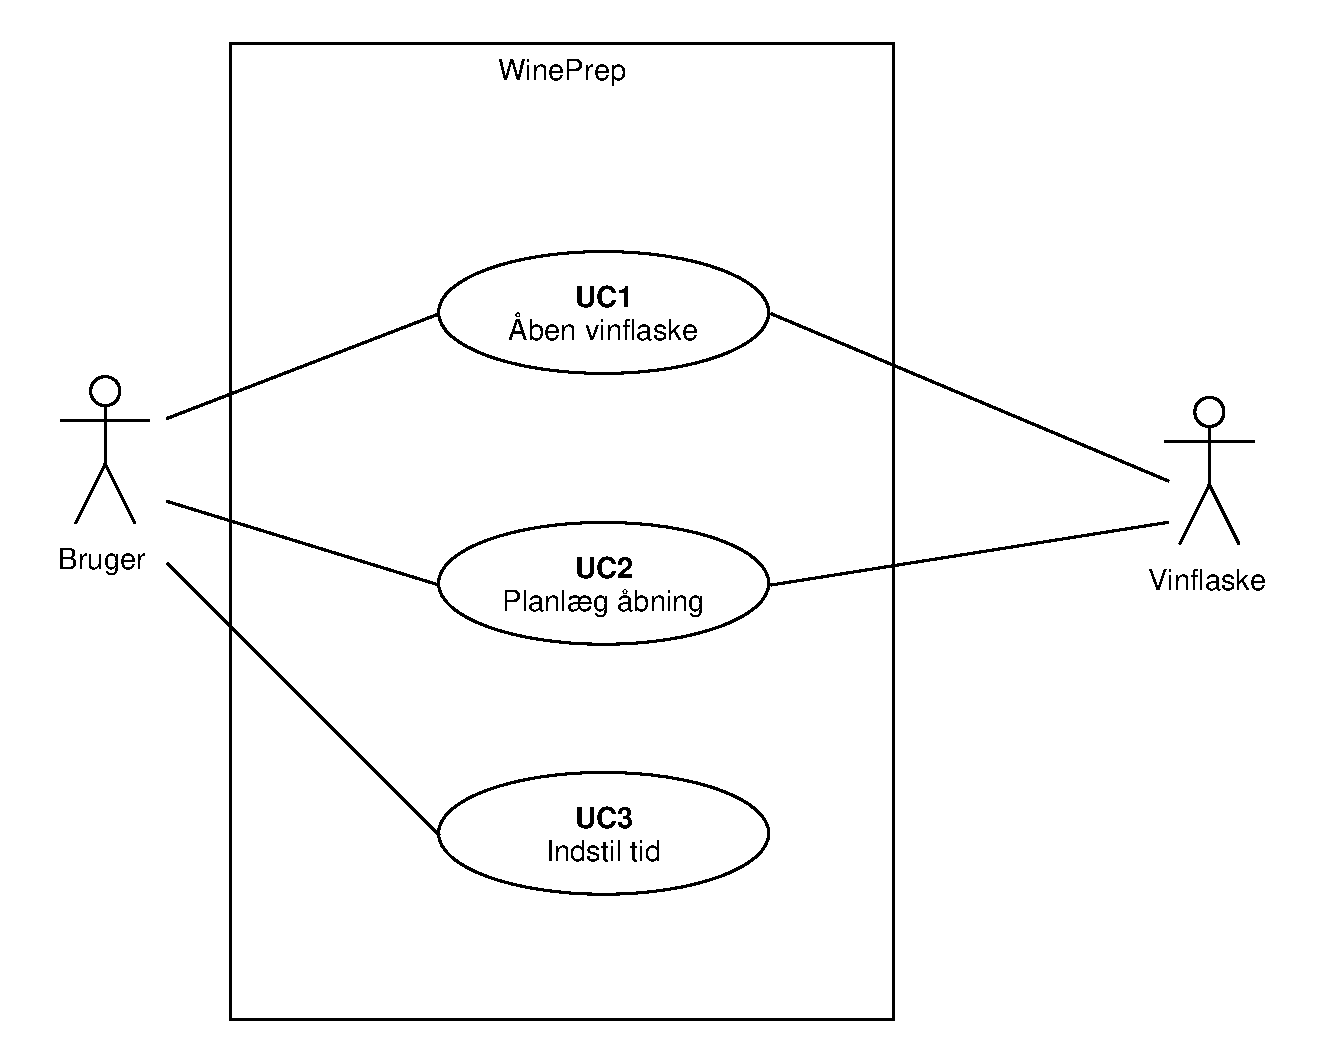
\includegraphics[scale=0.5]{usecasediagram.pdf}
\caption[Figur]{Use-case Diagram}
\end{figure}

\newpage
\subsection{Use-case 1: Åbn Vinflaske}
\rowcolors{1}{white}{lightgray}
\begin{tabular}{>{\bfseries}p{100pt} p{300pt}}
%	\caption[Tabel]{Fully dressed use-case 1}
	Navn & \bfseries{UC 1: Åbn Vinflaske} \\
	Mål & At åbne vinflasken og dermed tillade brugeren adgang til vinen\\
	Initiering & Bruger trykker \emph{Åbn nu} på brugergrænsefladen\\
	Aktører & Primær: Bruger \\
	Antal Samtidige forekomster & 1 \\
	Prækondition & Vinflasken er anbragt i maskinen og systemet er klar til brug. Desuden er vinflasken uåbnet og forseglingen er fjernet\\
	Postkondition & Vinflasken er åbnet og proppen er fjernet\\
	Hovedscenarie & \begin{enumerate}
		\item Bruger trykker Åbn nu på brugergrænsefladen
		\item System detekterer vinflaskens type og position
		\subitem [Ext. 1: System registrerer ugyldig type af vinflaske]
		\subitem [Ext. 2: System kan ikke registrere en vinflaske] 
		\item System låser vinflasken i dens position
		\item System fjerner prop fra vinflasken
		\item System frigiver vinflasken
		\item System meddeler brugeren om at vinflasken er åbnet og klar til brug.
		\item System dispenserer prop.
	\end{enumerate} \\
	Udvidelser/Undtagelser & 
	\begin{enumerate}{}{}
	\item[Ext.1] System registrerer ugyldig type af vinflaske
		\subitem[1.1] System meddeler brugeren om at typen af vinflaske er ugyldig.
		\subitem[1.2] UC1 Afsluttes.
	\item[Ext.2] System kan ikke registrere en vinflaske
		\subitem[2.1] {System meddeler brugeren om at ingen vinflaske \newline er
		registreret
}
		\subitem[2.2] UC afsluttes
	\end{enumerate}\\
\end{tabular}

\pagebreak

\subsection{Use-case 2: Planlæg Åbning}
\rowcolors{1}{white}{lightgray}
\begin{longtable}{>{\bfseries}p{100pt} p{300pt}}
	
	Navn & \bfseries{UC 2: Planlæg Åbning} \\
	Mål & Vinen er drikkeklar til et forudbestemt tidspunkt\\
	Initiering & Bruger trykker Planlæg åbning-knappen på brugergrænsefladen\\
	Aktører & Primær: Bruger \\
	Antal Samtidige forekomster & 1 \\
	Prækondition & Vinflasken er anbragt i systemet og systemet er klar til brug. Desuden er vinflasken uåbnet og forseglingen er fjernet. \\
	Postkondition & Vinflasken er drikkeklar til det valgte tidspunkt\\
	Hovedscenarie & \begin{enumerate}
		\item Bruger trykker Planlæg åbning-knappen på brugergrænsefladen	
		\item Bruger vælger tidspunkt på systemet
		\subitem [Ext. 1: Bruger ønsker ikke at åbne vin] 
		\item Bruger bekræfter valgt tidspunkt
		\subitem [Ext. 2: Vinen kan ikke iltes korrekt til det valgte tidspunkt]
		\item System venter til iltningstidspunktet
		\subitem [Ext. 5: Bruger annullerer planlagt åbning af vin]
		\item fortsæt med Usecase 1	
	\end{enumerate} \\
	Udvidelser/Undtagelser & 
	\begin{enumerate}
		\item[Ext.1] Bruger ønsker ikke at åbne vin
		
		\subitem[1.1a] Bruger trykker på tilbage
		\subitem[1.2b] UC afsluttes
		\item[Ext.2] Vinen kan ikke iltes korrekt til det valgte tidspunkt
		\subitem[2.1] System beder bruger bekræfte valg af tidspunkt
		\subitem[2.2a] Bruger trykker bekræft
		\subitem[2.3a] UC fortsættes fra punkt 1 i UC 1
		\subitem[2.2b] bruger trykker annuller
		\subitem[2.3b] UC afsluttes
		\item[Ext.3] System registrerer ugyldig type af vinflaske
		\subitem[3.1] System meddeler brugeren om at typen af vinflaske er ugyldig.
		\subitem[3.2] UC1 Afsluttes.
		\item[Ext.4] System kan ikke registrere en vinflaske
		\subitem[4.1] {System meddeler brugeren om at ingen vinflaske \newline er
		registreret}
		\item[Ext.5] Bruger annullerer planlagt åbning af vin
		\subitem[5.1] Bruger trykker stop
		\subitem[5.2] System beder bruger bekræfte valg
		\subitem[5.3] Bruger trykker bekræft
	\end{enumerate}
\end{longtable}

\begin{longtable}{>{\bfseries}TX TX}
%	\caption[Tabel]{Fully dressed use-case 1}
	Navn & \bfseries{\nameref{UC3}} \\
		Mål & At indstille tiden på systemets indbyggede ur\\
	Initiering & Bruger vælger indstillinger \\
	Aktører & Primær: Bruger \\
	Antal Samtidige forekomster & 1 \\
	Prækondition & Bruger befinder sig i hovedmenuen \\
	Postkondition & Tiden er indstillet korrekt \\
	Hovedscenarie & \begin{enumerate}
		\item Bruger trykker på indstillinger
		\item Bruger trykker på dropdownmenu for timer.
		\item Bruger vælger antal timer.
		\item System gør bekræftelsesknappen tilgængelig.
		\item Bruger trykker på dropdownmenu for minutter.
		\item Bruger vælger antal minutter.
		\item Bruger trykker på bekræftelsesknappen 
		\subitem [Ext. 1:Bruger trykker på tilbageknap.]
		\item System viser valgt klokkeslet på brugergrænsefladen
		
	\end{enumerate} \\
	Udvidelser/Undtagelser & 
	\begin{enumerate}{}{}
	\item[Ext.1]:Bruger trykker på tilbageknap.
	
		\subitem[1.1] Bruger trykker på tilbageknappen.
		\subitem[1.2] System kommer tilbage til hovedmenu.	 
		\subitem[1.3]UC afsluttes. \newline 
	\end{enumerate}
\end{longtable}
\pagebreak